\documentclass{beamer}
\usetheme{Berkeley}
\definecolor{UBCblue}{RGB}{25,25,112} % UBC Blue (primary)
\usecolortheme[named=UBCblue]{structure}

\usepackage{ebproof}
\usepackage{forest}
\usepackage{simplebnf}
\usepackage{graphicx}
\usepackage{listings}
\usepackage{tcolorbox}
\usepackage[backend=biber,style=numeric-comp,sorting=none]{biblatex}

\addbibresource{./bib/refs.bib}

\AtBeginBibliography{\footnotesize}

\AtEveryBibitem{%
  \clearfield{doi}%
  \clearfield{url}%
  \clearfield{note}%
  \clearfield{issn}%
  \clearfield{isbn}%
}

\definecolor{bluekeywords}{rgb}{0.13, 0.13, 1}
\definecolor{greencomments}{rgb}{0, 0.5, 0}
\definecolor{redstrings}{rgb}{0.9, 0, 0}
\definecolor{graynumbers}{rgb}{0.5, 0.5, 0.5}

\lstset{
    columns=fullflexible,
    showspaces=false,
    showtabs=false,
    breaklines=true,
    showstringspaces=false,
    breakatwhitespace=true,
    escapeinside={(*@}{@*)},
    commentstyle=\color{greencomments},
    keywordstyle=\color{bluekeywords},
    stringstyle=\color{redstrings},
    numberstyle=\color{graynumbers},
    basicstyle=\ttfamily\scriptsize,
    frame=l,
    framesep=12pt,
    xleftmargin=12pt,
    tabsize=4,
    captionpos=b
}

\graphicspath{ {./res/} }

\setbeamertemplate{footline}[frame number]

\usefonttheme[onlymath]{serif}

%Information to be included in the title page:
\title{Optimisation de la vitesse de compilation par la fusion entre inférence de types et analyse syntaxique}
\author{Enogad Le Biavant--Frederic}
\institute{Alain René Lesage MPI}
\date{2025}

\begin{document}

\frame{\titlepage}

\section{Présentation générale}
\begin{frame}
		\frametitle{L'idée}
		Karm, 2022
		\begin{center}
				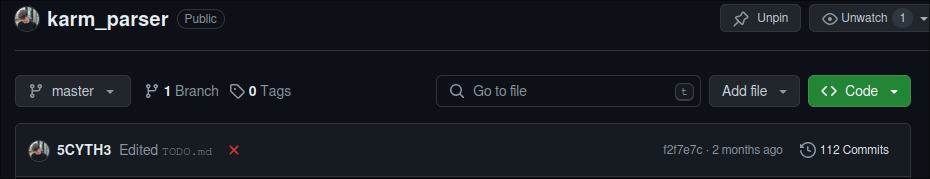
\includegraphics[scale=0.25]{repo}
		\end{center}
		Comment optimiser la vitesse de compilation en fusionnant analyse syntaxique et sémantique ?
\end{frame}

\begin{frame}[fragile]
		\frametitle{L'idée}

		$\Gamma = \{ 
				\only<1->{\texttt +: int \rightarrow int \rightarrow int}
				\only<2->{,\; \texttt x: \tau}
		\}$
		\\
		$\texttt{let} \; succ = \lambda x.(+ \; x \; 1)$
		
		\begin{columns}
				\begin{column}{0.5\textwidth}
						\begin{center}
						\begin{forest}
								for tree = {
										edge = {<-, semithick},
								}
								[succ
										[x]
										[+, name=spec +
												[x]
												[1]	
										]
								]
						\end{forest}
						\end{center}
				\end{column}
				\begin{column}{0.5\textwidth}
						\begin{center}
						\begin{forest}
								for tree = {
										edge = {<-, semithick},
								}
								[succ
								[x,edge label={node[midway, left]{\only<1->{$\{x:\tau\}$}}}]
										[+,edge label={node[midway, right]{\only<3->{$\{\tau = int\}$}}}
												[x, edge label={node[midway, left]{\only<2->{$\{x:\tau\}$}}}]
												[1]	
										]
								]
						\end{forest}
						\end{center}
				\end{column}
		\end{columns}
		\only<4>{Parsing récursif descendant}
\end{frame}

\section{Définitions}
\subsection{Parsing}
\begin{frame}
		\frametitle{Grammaire}
		\begin{bnf}
				$program$ ::= $expr$;;
				$expr$ ::= | $abs$ | $app$ | $letbinding$;;
				$app$ ::= $term$ [\{ $term$ \}];;
				$abs$ ::= "$\backslash$" $id\space$ "." $\space expr$;;
				$letbinding$ ::= "let" $id$ "=" $expr$ "in" $expr$;;
				$term$ ::= | \texttt{string} | \texttt{int} | \texttt{bool} | $id$ | "(" $expr$ ")"
		\end{bnf} 
\end{frame}

\subsection{Théorie des types}
\begin{frame}
		\frametitle{TT - Définitions}
		Définition de Type : classification de termes (Church).\\
		Théorie de travail : Lambda calcul simplement typé (LCST), polymorphique.\\
		\[
				\texttt{let\;} id = \lambda x.x :\forall \sigma\to\sigma
		\]
\end{frame}

\begin{frame}
\frametitle{Hindley-Milner}
		\[
		\begin{prooftree}
				\hypo{x:\sigma\in\Gamma}
				\infer1[var]{\Gamma \vdash x:\sigma}
		\end{prooftree}
		\]
		\newline
		\[
		\begin{prooftree}
				\hypo{\Gamma, x:\tau \vdash e:\tau'}
				\infer1[abs]{\Gamma \vdash \lambda x.e:\tau \to \tau'}
		\end{prooftree}
		\]
		\newline
		\[
		\begin{prooftree}
				\hypo{\Gamma \vdash f:\tau \to \tau'}
				\hypo{\Gamma \vdash e : \tau}
				\infer2[app]{\Gamma \vdash f\ e : \tau'}
		\end{prooftree}
		\]
\end{frame}

\begin{frame}
		\frametitle{Hindley-Milner}
		Algorithme W
		\begin{columns}
				\begin{column}{0.5\textwidth}
						\begin{enumerate}
								\item Assignation de variables de types aux expressions
								\item Génération de contraintes
								\item Substitutions
								\item Unification
								\item Instantiation, généralisation
						\end{enumerate}
				\end{column}
				\begin{column}{0.5\textwidth}
						\begin{forest}
								for tree = {
										edge = {<-, semithick},
								}
								[succ
								[x,edge label={node[midway, left]{$\{x:\tau\}$}}]
										[expr,edge label={node[midway, right]{$\{expr:\beta\}$}}
												[+,edge label={node[midway, left]{$\{\beta = int, \tau = int\}$}}
														[x, edge label={node[midway, left]{$\{x:\tau\}$}}]
														[1]	
												]
										]
								]
						\end{forest}
				\end{column}
		\end{columns}
\end{frame}

\section{Résultats}
\begin{frame}[t]
		\frametitle{Résultats}
		
		\begin{center}
				$\mathcal W : \tilde \Gamma \times Expr \to Subst \times Type$\\
				$\mathcal W^* : \tilde \Gamma \times L \to Subst \times \Gamma \times Expr \times L $	
		\end{center}
		
		Machine : i7 5th gen 3.00Ghz\\
		\vspace{5mm}
		Fichier de test : 1000 premiers nombres de church\\
		Version non optimisée : $\approx 26.37s$\\
		Version optimisée : $\approx 3.88s$\\
		\vspace{5mm}
		Fichier de test : 10K application de fonction successeur\\
		Version non optimisée : $\approx 1.48s$\\
		Version optimisée : $\approx 1.51s$
\end{frame}

\begin{frame}
		\frametitle{Résultats}
		\begin{center}
				% \includegraphics[scale=0.25]{graph}
		\end{center}
\end{frame}


\section{Conclusion}
\begin{frame}
		\frametitle{Conclusion}
		\begin{tcolorbox}[title=Bénéfices]
				Durée inférieure lorsque beaucoup d'unifications
		\end{tcolorbox}
		\begin{tcolorbox}
				Plus permissif envers les grammaires très imbriquées que les systèmes traditionnels
		\end{tcolorbox}
\end{frame}

\section{Formalisation}
\begin{frame}
		\frametitle{Formalisation}
		Automates d'arbres : $\mathcal A  = (\mathcal F, Q, Q_f, \Delta)$\\
		\begin{itemize}
				\item{$\mathcal F$ : Alphabet gradué (fonction d'arité $ar$) }
		\end{itemize}
		On peut décrire la grammaire comme une NRTG
\end{frame}

\section{Bibliographie}
\begin{frame}
		\frametitle{Bibliographie}
		\nocite{*}
		\printbibliography
\end{frame}

\section{Annexe}
\begin{frame}[fragile]
		\frametitle{Annexe - Lexemes}
		\begin{lstlisting}[language=ML]
type literal = 
    | Str of string
    | Int of int
    | Bool of bool
    [@@deriving show]

type t =
    | Let
    | Lambda
    | Dot
    | Assign
    | In
    | LParen
    | RParen
    | Id of string
    | Literal of literal
    [@@deriving show]

type program = t list
[@@deriving show]
		\end{lstlisting}
\end{frame}

\begin{frame}[fragile]
		\frametitle{Annexe - Expressions}
		\begin{lstlisting}[language=ML]
type literal =
    | Str of string
    | Int of int
    | Bool of bool
[@@deriving show]

type t =
    | Var of string
    | Abs of string * t
    | App of t * t
    | Let of string * t * t
    | Literal of literal
[@@deriving show]
		\end{lstlisting}
\end{frame}

\begin{frame}[fragile]
		\frametitle{Annexe - Types}
		\begin{lstlisting}[language=ML]
type t =
    (* Primitives *)
    | Bool
    | Str
    | Int
    | TVar of string
    (* Function *)
    | Abs of t * t (* @-> *)
    (* Scheme *)
    | Forall of string * t 
    [@@deriving show];;

let ( @-> ) t1 t2 = Abs (t1, t2)

let counter = ref 0;;

let fresh_tv () =
    let v = "t" ^ string_of_int !counter in
    incr counter;
    TVar v
let reset_tv_counter () = counter := 0;;

		\end{lstlisting}

\end{frame}

\begin{frame}[fragile]
		\frametitle{Annexe - Types}
		\begin{lstlisting}[language=ML]
module TypeMap = Map.Make(String)

type subst = t TypeMap.t (* // *)

let rec apply_subst (s: subst) (t: t) =
    match t with
    | TVar v -> begin
        match TypeMap.find_opt v s with (* If type is not found, works like Id *)
        | Some x -> x
        | None -> t
    end
    | Abs (arg, ret) -> Abs (apply_subst s arg, apply_subst s ret)
    | Forall (v, t) -> Forall (v, apply_subst (TypeMap.remove v s) t)
    | t -> t

let ( *&* ) s1 s2 =
    TypeMap.union (fun _ t _ -> Some t) (TypeMap.map (apply_subst s1) s2) s1
		\end{lstlisting}
\end{frame}

\begin{frame}[fragile]
		\frametitle{Annexe - Types}
		\begin{lstlisting}[language=ML]
type env = t TypeMap.t;; (* String : Type *)

let extend_env env k t = TypeMap.add k t env

let apply_env (env: env) k: t =
    try TypeMap.find k env
    with Not_found -> failwith ("Var not in scope : " ^ k)

let apply_subst_to_env subst env = TypeMap.map (fun t -> apply_subst subst t) env;;
		\end{lstlisting}
\end{frame}

\begin{frame}[fragile]
		\frametitle{Annexe - Types}
		\begin{lstlisting}[language=ML]
module Ftv = Set.Make (String);;

type ftvs = Ftv.t

let rec free_tvs t: ftvs =
    match t with
    | Int | Bool | Str -> Ftv.empty
    | TVar v -> Ftv.singleton v
    | Abs (t1, t2) -> Ftv.union (free_tvs t1) (free_tvs t2)
    | Forall (v, t) -> Ftv.remove v (free_tvs t)

let free_tvs_env env =
    TypeMap.fold (fun _ t acc -> Ftv.union (free_tvs t) acc) env Ftv.empty
		\end{lstlisting}
\end{frame}

\begin{frame}[fragile]
		\frametitle{Annexe - Types}
		\begin{lstlisting}[language=ML]
exception TypeError of string

let rec unify t1 t2: subst =
    match t1, t2 with
    | Bool, Bool | Int, Int | Str, Str -> TypeMap.empty
    | TVar v1, TVar v2 when v1 = v2 -> TypeMap.empty
    | TVar v, t | t, TVar v ->
        if Ftv.mem v (free_tvs t) then
            raise (TypeError ("Occurs check failed for variable " ^ v))
        else
            TypeMap.singleton v t
    | Abs (t1a, t1b), Abs (t2a, t2b) ->
        let s1 = unify t1a t2a in
        let s2 = unify (apply_subst s1 t1b) (apply_subst s1 t2b) in
        s2 *&* s1
    | Forall (v1, t1), Forall (v2, t2) ->
        let t2' = apply_subst (TypeMap.singleton v2 (TVar v1)) t2 in
        unify t1 t2'
    | _ -> raise (TypeError "Cannot unify types")
		\end{lstlisting}
\end{frame}

\begin{frame}[fragile]
		\frametitle{Annexe - Types}
		\begin{lstlisting}[language=ML]
let generalize env t =
    let env_fv = free_tvs_env env in
    let ftvs_of_t = free_tvs t in
    let vars_to_generalize = Ftv.filter (fun v -> not (Ftv.mem v env_fv)) ftvs_of_t in
    match Ftv.elements vars_to_generalize with
    | [] -> t
    | vars -> List.fold_right (fun v acc -> Forall (v, acc)) vars t

let rec instantiate t =
    match t with
    | Forall (v, t) -> let fresh_var = fresh_tv () in instantiate (apply_subst (TypeMap.singleton v fresh_var) t)
    | _ -> t
		\end{lstlisting}
\end{frame}

\begin{frame}[fragile]
		\frametitle{Annexe - Parsing classique}
		\begin{lstlisting}[language=ML]
type traversal = {
    expr: Expr.t;
    rest: Token.program;
}

let match_literals = function
    | Token.Str s -> Expr.Literal (Expr.Str s)
    | Token.Int i -> Expr.Literal (Expr.Int i)
    | Token.Bool b -> Expr.Literal(Expr.Bool b)

let rec parse_expr (program: program): traversal =
    match program with
    | Lambda :: Id arg :: Dot :: rest ->
        let { expr = body; rest = rest'; } = parse_expr rest in 

        {
            expr = Abs (arg, body);
            rest = rest';
        }
    | Let :: _ -> parse_let program
    | _ -> parse_app program
		\end{lstlisting}
\end{frame}

\begin{frame}[fragile]
		\frametitle{Annexe - Parsing classique}
		\begin{lstlisting}[language=ML]
and parse_let (program: program): traversal =
    match program with
    | Let :: Id i :: Assign :: t -> 
        let { expr = body; rest; } = parse_expr t in

        let { expr = in_expr; rest = rest'; } = parse_ins rest in

        {
            expr = Let (i, body, in_expr);
            rest = rest';
        }
    | _ -> failwith "Expected `Let`."
		\end{lstlisting}
\end{frame}
\begin{frame}[fragile]
		\frametitle{Annexe - Parsing classique}
		\begin{lstlisting}[language=ML]
and parse_ins (program: program): traversal =
    match program with
    | In :: t -> parse_expr t
    | _ -> failwith "No 'in' clause given. "

and parse_parenthesized (program: program): traversal =
    match program with
    | LParen :: t -> begin
        let e = parse_expr t in
        match e.rest with
        | RParen :: t' -> { expr = e.expr; rest = t'; }
        | _ -> failwith "Unclosed parenthesis"
    end
    | _ -> failwith "Expected LParen."
		\end{lstlisting}
\end{frame}

\begin{frame}[fragile]
		\frametitle{Annexe - Parsing classique}
		\begin{lstlisting}[language=ML]
and parse_app (program: program): traversal = 
    let rec aux (lhs: traversal) = 
        let { expr = lhs_expr; rest; } = lhs in

        match rest with
        | [] | In :: _ | RParen :: _ -> lhs
        | _ -> begin
            let { expr = rhs_expr; rest = rest'; } = parse_term rest in
            
            let res = {
                expr = App (lhs_expr, rhs_expr);
                rest = rest';
            } in
            aux res
        end
    in 
    let initial = parse_term program in
    aux initial
		\end{lstlisting}
	
\end{frame}
\begin{frame}[fragile]
		\frametitle{Annexe - Parsing classique}
		\begin{lstlisting}[language=ML]
and parse_term (program: program): traversal =
    match program with
    | Id x :: rest -> 
        { 
            expr = Var x; 
            rest;
        }
    | Token.Literal l :: t -> 
        {
            expr = match_literals l;
            rest = t;
        }  
    | LParen :: _ -> parse_parenthesized program
    | RParen :: _ -> failwith "Alone RParen. ?"
    | _ -> failwith "Unexpected token"
		\end{lstlisting}
	
\end{frame}
\begin{frame}[fragile]
		\frametitle{Annexe - Parsing classique}
		\begin{lstlisting}[language=ML]
let parse (program: program) =
		let { expr; rest = _; } = parse_expr program in
    expr
;;

let type_of_literal = function
    | Expr.Str _ -> Types.Str
    | Expr.Bool _ -> Types.Bool
    | Expr.Int _ -> Types.Int
;;
		\end{lstlisting}
\end{frame}
\begin{frame}[fragile]
		\frametitle{Annexe - Parsing classique}
		\begin{lstlisting}[language=ML]
let rec infer_types_aux env e cont = 
    let open Types in
    match e with
    | Expr.Literal l ->
        let t = type_of_literal l in
        cont (t, TypeMap.empty)
    | Var x ->
        let t = apply_env env x in
        cont (t, TypeMap.empty)
    | Abs (x, e) ->
        let t = fresh_tv () in
        let env' = extend_env env x t in
        infer_types_aux env' e (fun (t', s) ->
            let t_res = (apply_subst s t) @-> t' in
            cont (t_res, s)
        )
    
		\end{lstlisting}
\end{frame}
\begin{frame}[fragile]
		\frametitle{Annexe - Parsing classique}
	
		\begin{lstlisting}[language=ML]
	| App (e1, e2) ->
        infer_types_aux env e1 (fun (t1, s1) ->
            let env' = apply_subst_to_env s1 env in
            infer_types_aux env' e2 (fun (t2, s2) ->
                let tv = fresh_tv () in
                let s3 = unify (apply_subst s2 t1) (t2 @-> tv) in
                let f_subst = s3 *&* s2 *&* s1 in
                cont (apply_subst f_subst tv, f_subst)
            )
        )
    | Let (x, e1, e2) ->
        infer_types_aux env e1 (fun (t1, s1) ->
            let t' = generalize env (apply_subst s1 t1) in
            let env' = extend_env env x t' in
            infer_types_aux env' e2 (fun (t2, s2) ->
                cont (t2, s2 *&* s1)
            )
        )
		\end{lstlisting}
\end{frame}
\begin{frame}[fragile]
		\frametitle{Annexe - Parsing classique}
		\begin{lstlisting}[language=ML]
				
let infer_types env e =
		infer_types_aux env e (fun res -> res)

let run (p: program) (env: Types.env) =
    let ast = parse p in
    let t, _ = infer_types env ast in
    (ast, t)
;;
		\end{lstlisting}
\end{frame}

\begin{frame}[fragile]

		\frametitle{Annexe - Parsing fusionné}
		\begin{lstlisting}[language=ML]

type traversal = {
    expr: Expr.t;
    t: Types.t;
    subst: Types.subst;
    rest: Token.t list;
}

let match_literals = function
    | Token.Str s -> Literal (Str s)
    | Token.Int i -> Literal (Int i)
    | Token.Bool b -> Literal(Bool b)

let type_literals = function
    | Token.Str _ ->  Types.Str
    | Token.Int _ -> Types.Int
    | Token.Bool _ -> Types.Bool

let fresh_id (id: string) (env: Types.env): Types.t * Types.env = 
    let tv = Types.fresh_tv () in
    let env' = Types.extend_env env id tv in
    (tv, env')
		\end{lstlisting}
	
\end{frame}
\begin{frame}[fragile]
		\frametitle{Annexe - Parsing fusionné}
		\begin{lstlisting}[language=ML]
let rec parse_expr (program: Token.t list) (env: Types.env): traversal =
    match program with
    | Lambda :: Id arg :: Dot :: rest ->
        let (tv, env') = fresh_id arg env in
        let { expr = body; t; subst; rest = rest'; } = parse_expr rest env' in 

        {
            expr = Abs (arg, body);
            t = Types.Abs (Types.apply_subst subst tv, t);
            subst;
            rest = rest';
        }
    | Let :: _ -> parse_let program env
    | _ -> parse_app program env
		\end{lstlisting}
	
\end{frame}
\begin{frame}[fragile]
		\frametitle{Annexe - Parsing fusionné}
		\begin{lstlisting}[language=ML]
			
and parse_let (program: Token.t list) (env: Types.env): traversal =
    match program with
    | Let :: Id i :: Assign :: t -> 
        let open Types in
        let { expr = body; t = t1; subst = subst1; rest; } = parse_expr t env in
        let t' = generalize env (apply_subst subst1 t1) in (* Get the type of the let def *)
        let env' = extend_env env i t' in (* Add the typesig of the let-expr to the ctx *)

        let { expr = in_expr; t = t2; subst = subst2; rest = rest'; } = parse_ins rest env' in

        {
            expr = Let (i, body, in_expr);
            t = t2;
            subst = subst2 *&* subst1;
            rest = rest';
        }
    | _ -> failwith "Expected `Let`."
		\end{lstlisting}
	
\end{frame}
\begin{frame}[fragile]
		\frametitle{Annexe - Parsing fusionné}
		\begin{lstlisting}[language=ML]
				
and parse_ins (program: Token.t list) (env: Types.env): traversal =
    match program with
    | In :: t -> parse_expr t env
    | _ -> failwith "No 'in' clause given. "

and parse_parenthesized (program: Token.t list) (env: Types.env): traversal =
    match program with
    | LParen :: t -> begin
        let e = parse_expr t env in
        match e.rest with
        | RParen :: t' -> { expr = e.expr; t = e.t; subst = e.subst; rest = t'; }
        | _ -> failwith "Unclosed parenthesis"
    end
    | _ -> failwith "Expected LParen."
		\end{lstlisting}
	
\end{frame}
\begin{frame}[fragile]
		\frametitle{Annexe - Parsing fusionné}
		\begin{lstlisting}[language=ML]
			
and parse_app (program: Token.t list) (env: Types.env): traversal = 
    let open Types in

    let rec aux (lhs: traversal) = 
        let { expr = lhs_expr; t = t1; rest; subst = s1; } = lhs in
        match rest with
        | [] | In :: _ | RParen :: _ -> lhs
        | _ -> begin
            let { expr = rhs_expr; t = t2; subst = s2; rest = rest'; } = parse_term rest env in
            let tv = fresh_tv () in
            let s3 = unify (apply_subst s2 t1) (Abs (t2, tv)) in 
            let f_subst = s3 *&* s2 *&* s1 in

		\end{lstlisting}
	
\end{frame}
\begin{frame}[fragile]
		\frametitle{Annexe - Parsing fusionné}
		\begin{lstlisting}[language=ML]
		   let res = {
                expr = App (lhs_expr, rhs_expr);
                t = apply_subst f_subst tv; 
                subst = f_subst;
                rest = rest';
            } in
            aux res
        end
    in 
    let initial = parse_term program env in
    aux initial
			
		\end{lstlisting}
	
\end{frame}
\begin{frame}[fragile]
		\frametitle{Annexe - Parsing fusionné}
		\begin{lstlisting}[language=ML]
			
and parse_term (program: Token.t list) (env: Types.env): traversal =
    match program with
    | Id x :: rest -> 
        let t = Types.apply_env env x in 
        { 
            expr = Var x; 
            t;
            subst = Types.TypeMap.empty; 
            rest;
        }
    | Token.Literal l :: t -> 
        {
            expr = match_literals l;
            t = type_literals l;
            subst = Types.TypeMap.empty;
            rest = t;
        }  
    | LParen :: _ -> parse_parenthesized program env
    | RParen :: _ -> failwith "Alone RParen. ?"
    | _ -> failwith "Unexpected token"
		\end{lstlisting}
	
\end{frame}
\begin{frame}[fragile]
		\frametitle{Annexe - Parsing fusionné}
		\begin{lstlisting}[language=ML]
			
let parse (program: Token.program) (env: Types.env) =
    Types.reset_tv_counter ();
    let { expr; t; subst = _; rest = _; } = parse_expr program env in
    (expr, t)
		\end{lstlisting}
	
\end{frame}
\end{document}
